\documentclass[oneside,a4paper,11pt,explicit]{book}
\usepackage[utf8]{inputenc}
\usepackage{icecream}
\usepackage[english]{babel}
\addto\captionsenglish{\renewcommand{\chaptername}{}}
\usepackage[accsupp]{axessibility}  % improves PDF readability for those with disabilities.
\usepackage[colorlinks = true,urlcolor  = blue,linkcolor = blue]{hyperref}
\usepackage{setspace}
\usepackage{listings}
\usepackage[most]{tcolorbox}
\usepackage{minitoc}


\renewcommand{\mtifont}{\large\sffamily}
\renewcommand{\mtcfont}{\small\sffamily}
\renewcommand{\mtcSfont}{\small\sffamily}
\renewcommand{\mtcSSfont}{\small\sffamily}
\renewcommand{\mtcSSSfont}{\small\sffamily}
\mtcsetpagenumbers{minitoc}{off} % turn off page numbering in minitocs
\addto{\captionsenglish}{% Making babel aware of special titles
	\renewcommand{\mtctitle}{Quick Links To Sections}
}
\setlength{\fboxrule}{5pt}
\setlength{\fboxsep}{4pt}

\definecolor{IceCreamLeaf}{HTML}{58743b}
\definecolor{IceCreamOrbit}{HTML}{732e00}
\definecolor{MACred}{rgb}{0.803921568627451, 0.3607843137254902, 0.3607843137254902}

\title{I.C.E.C.R.E.A.M. Tutorials}
\subtitle{\small Observing Earth from Above (Env 329) v24.06 \\
	\small Schmid College of Science and Technology, Chapman University}
\date{\today}

%% DOCUMENT
\setstretch{1.25}
\makeatletter
\begin{document}

\dominitoc

\faketableofcontents

\setcounter{chapter}{11} %Insert (Tutorial Number-1) Here; example for tutorial 4, enter 3

\chapter{Making Better Maps} %Enter Tutorial Name Here

\vspace{-2em}

\minitoc

\hrule

\vspace{1em}

\begin{tcolorbox}[enhanced,frame style image=blueshade.png,
	opacityback=0.75,opacitybacktitle=0.25,
	colback=blue!5!white,colframe=blue!75!black,title={\Large \textbf{Objectives:}}]
	\large
	\begin{enumerate}
		\item Familiarize yourself with the advanced map making features in QGIS, such as creating an inset and colorbrewer.
		\item Incorporate the ideas from the \href{https://www.observingearthfromabove.com/uploads/b/150001442-463159049665547396/davidoff_unedited_130.mp4}{Data Visualization} \& \href{https://www.observingearthfromabove.com/uploads/b/150001442-463159049665547396/jan_export_final_101.mp4}{Principles of Design} lectures.
	\end{enumerate}
\end{tcolorbox}

\clearpage 

%%%%%%%%%%%%%%%%%%%%%%%%%%%%%%%%%% Change Header to Have a Smaller Logo for Remainder of the Document
\fancyhead{}
\fancyhead[C]{\begin{tikzpicture}[overlay, remember picture]
		\fill[Blue2] (current page.north west) rectangle ($(current page.north east)+(0,-1in)$);
		\node[anchor=north west, text=white, font=\Large, minimum size=1in, inner xsep=5mm, align=left] at (current page.north west) {\bf{\MakeUppercase{\@title}}\\\@subtitle};
		\node[anchor=north east, minimum size=1in, inner xsep=5mm] at (current page.north east) {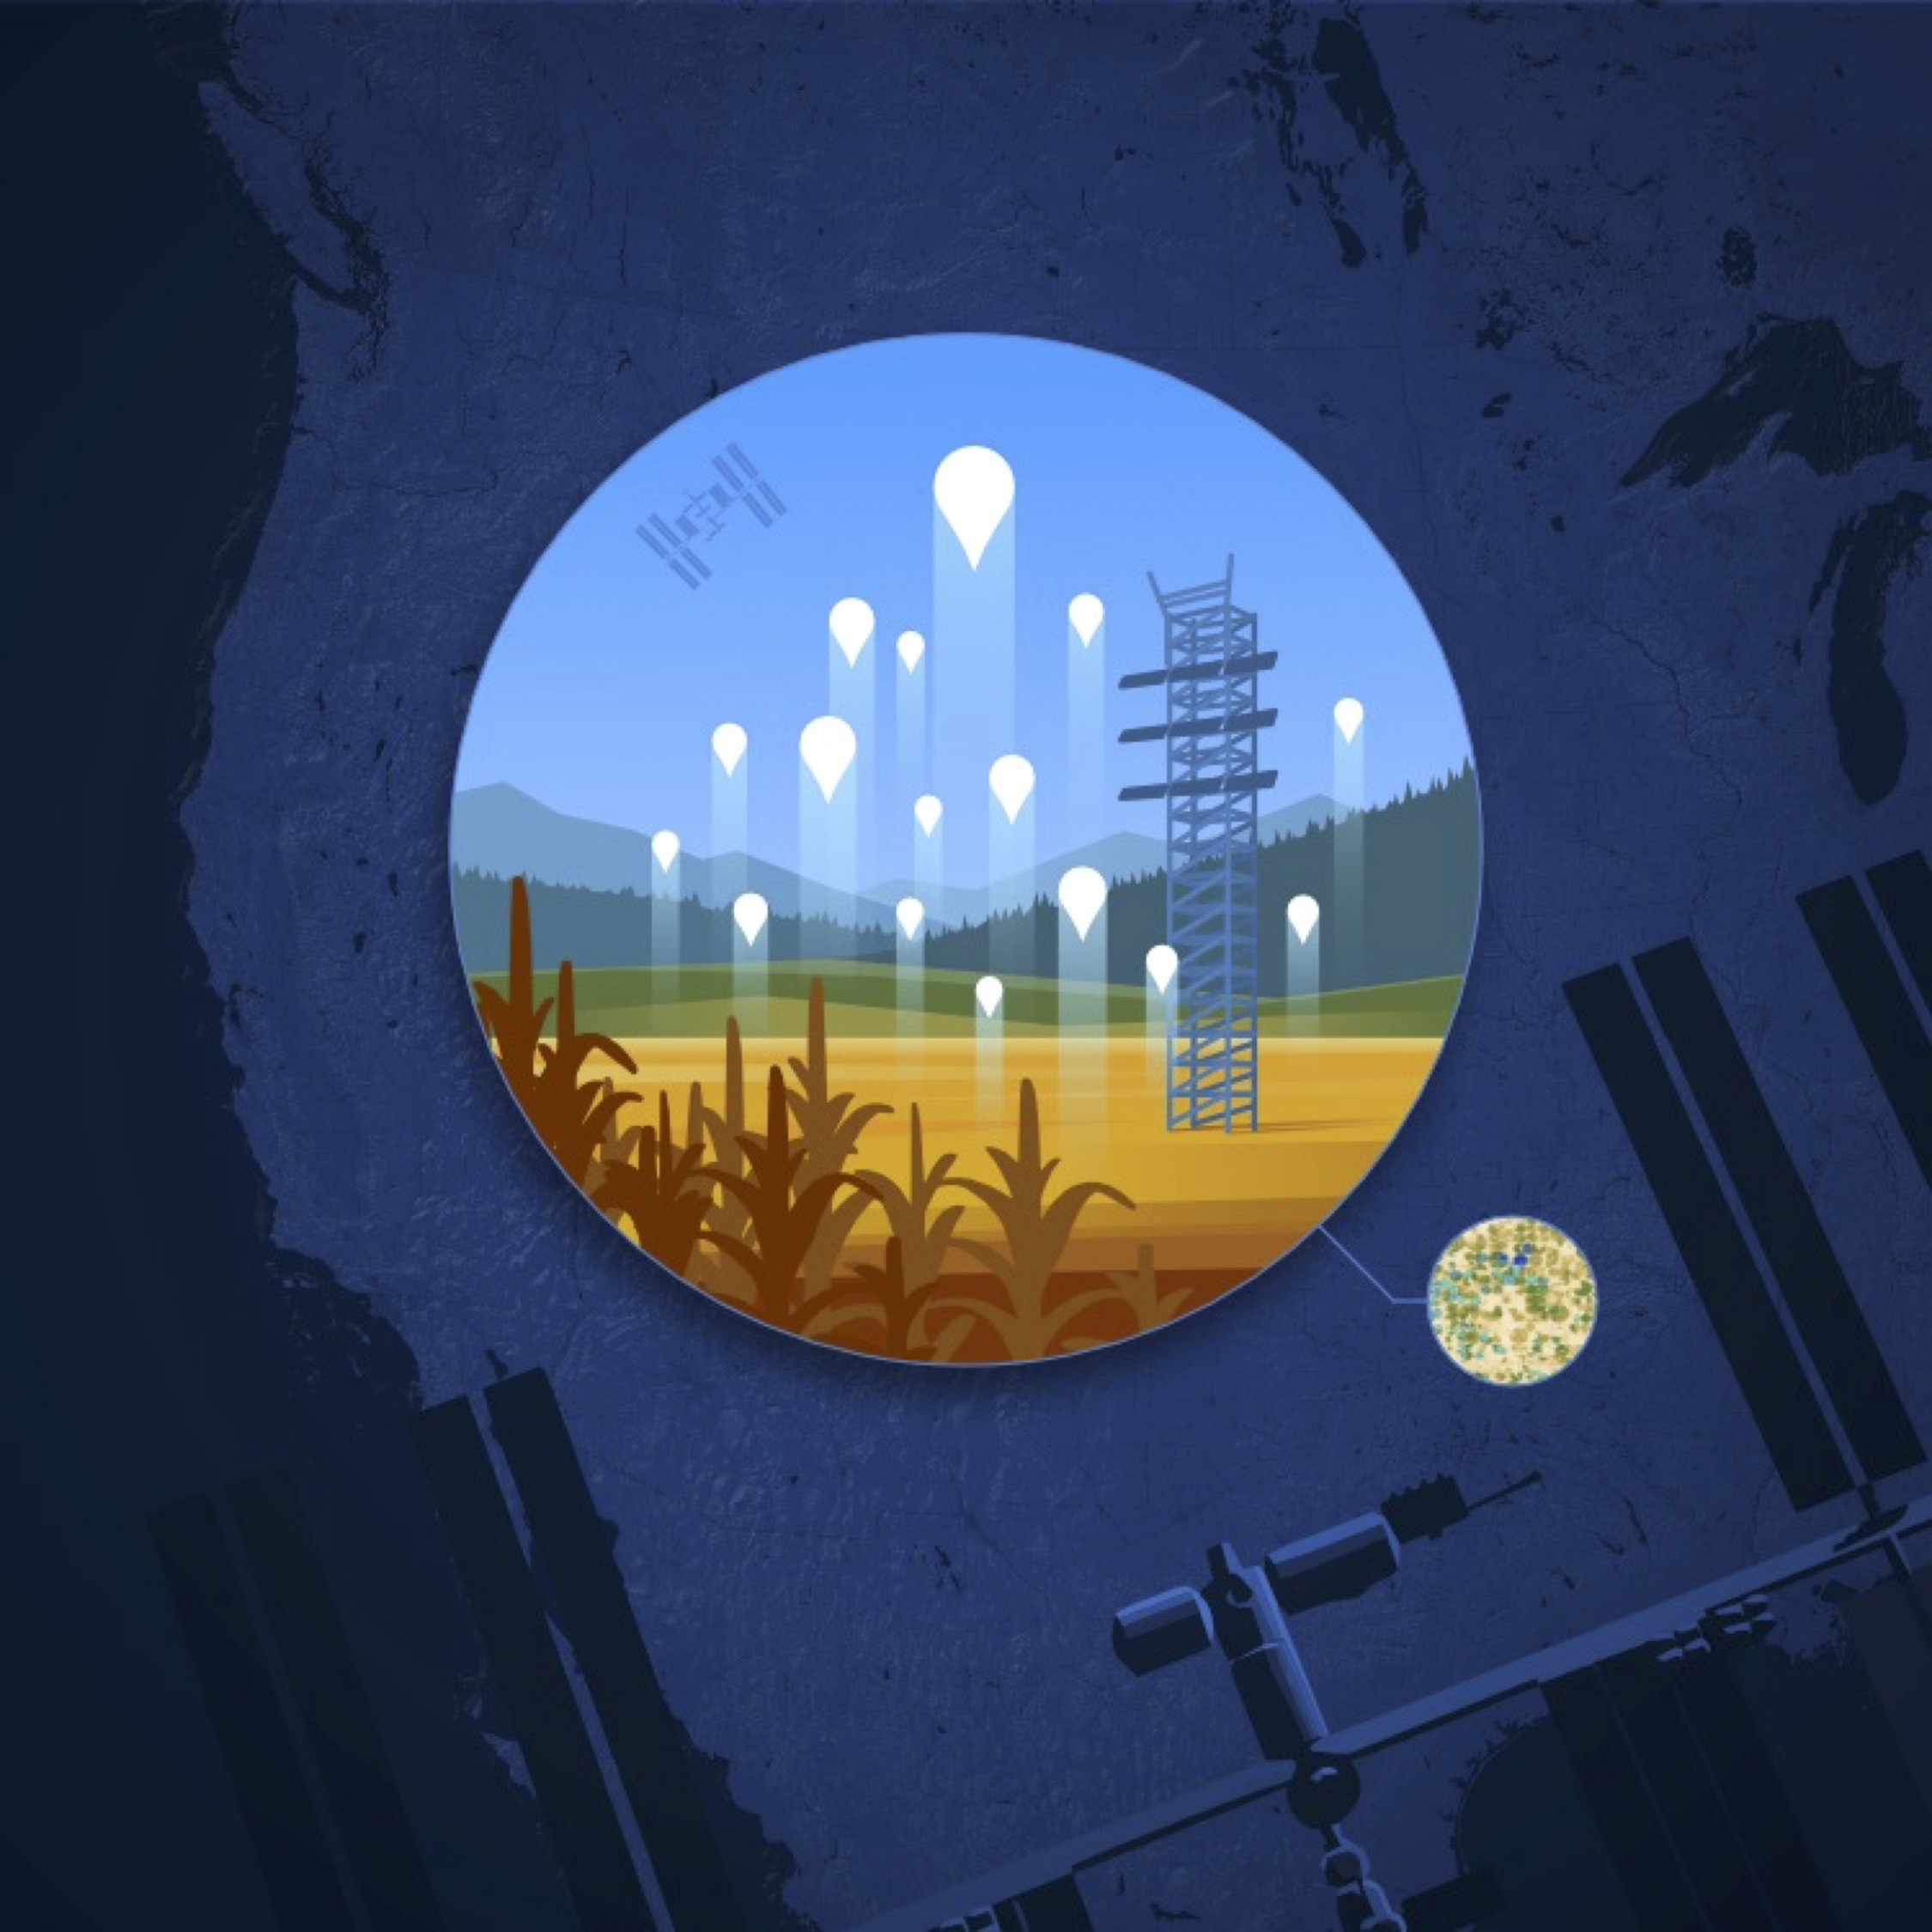
\includegraphics[scale=.03]{ECOSTRESS-BASE.jpg}};\end{tikzpicture}}
%%%%%%%%%%%%%%%%%%%%%%%%%%%%%%%%%%

\noindent\fbox{\begin{minipage}{.9665\textwidth}
			
	\vspace{1em}
	\begin{center}
		\textbf{\Large \underline{Motivation For Today's Tutorial: Impactful Map Making}}
	\end{center}
	
	\addcontentsline{toc}{section}{Motivation : Impactful Map Making}

	\vspace*{-1 em}
	
	\centerline{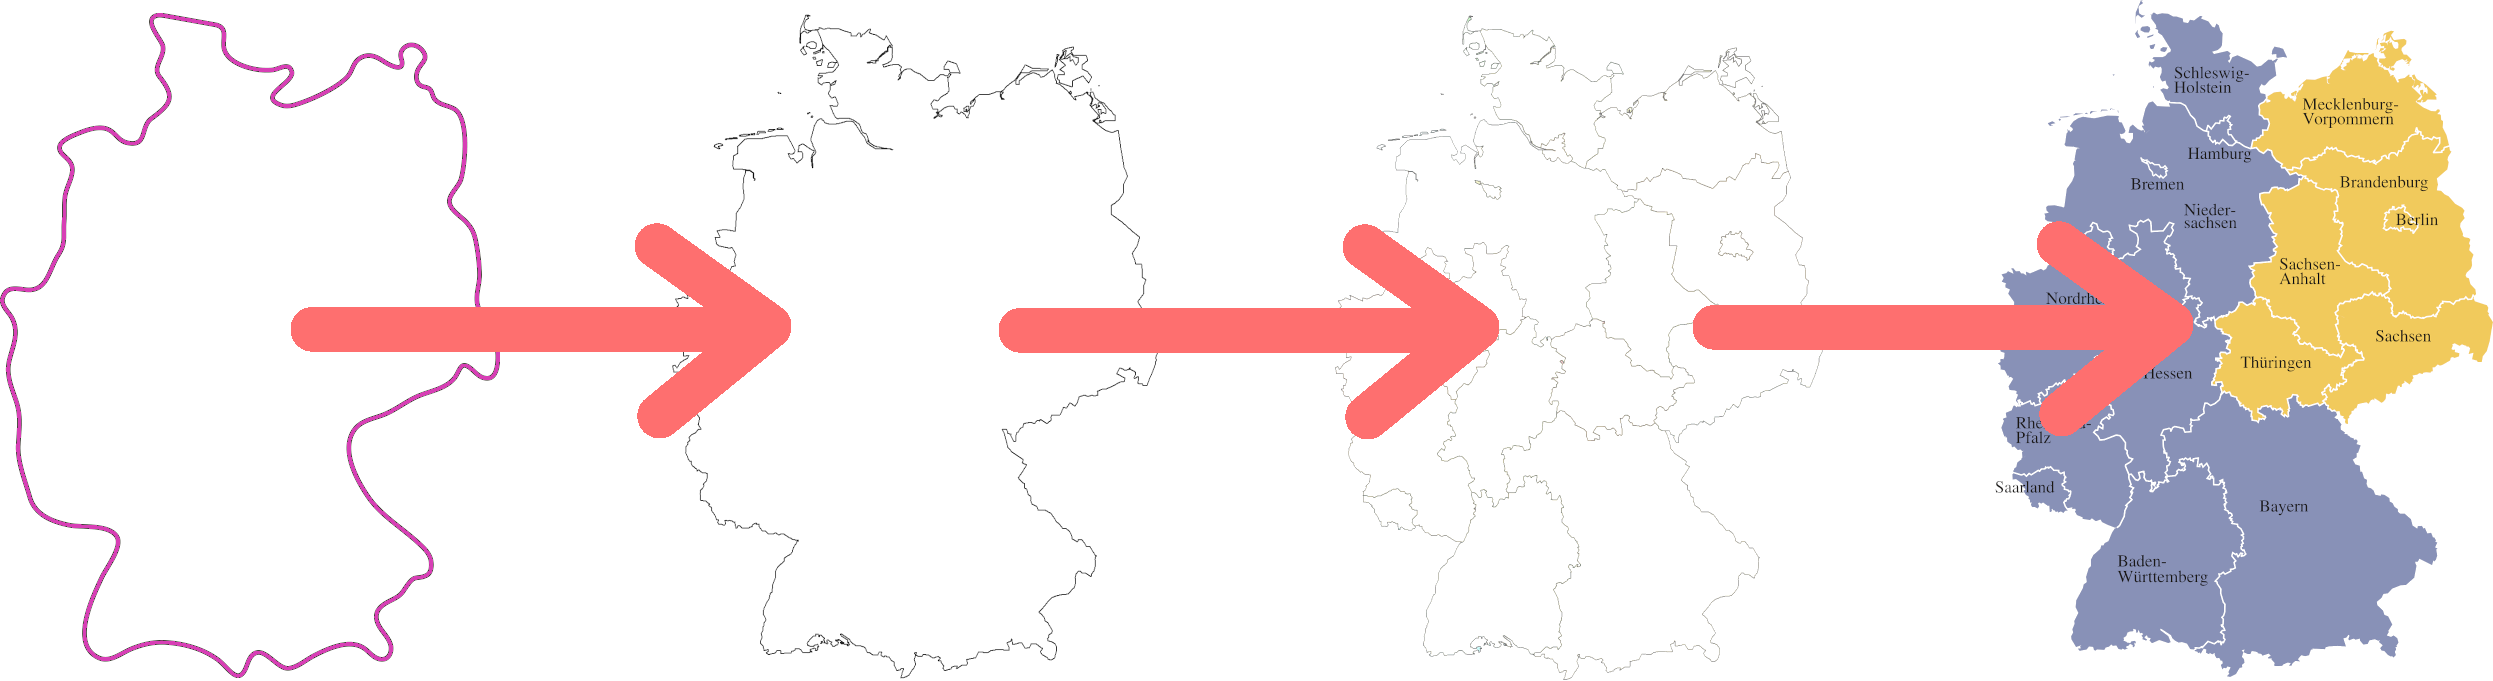
\includegraphics[width=\textwidth]{MakeBetterMaps.png}}
 
 What makes a great map? A great map clearly communicates its message to the reader. It should be easy to get oriented, determine distances and directions, and interpret the elements of the map. Although unintended conclusions are often blamed on data quality issues, misunderstandings are often the result of a miscommunication between the map creator and the audience (Mocnik 2022). Since our ultimate goal is to create influential maps for NASA press releases, it is a good time to refine our map-making skills to ensure that we are communicating the idea we want to communicate. To that end, today's tutorial shows off the more advanced map making skills we can do with QGIS and almost acts as a sequel to the bingeworthy hit blockbuster \href{https://jeremydforsythe.github.io/icecream-tutorials/Tutorial7_AddingElementsToMaps1/Tutorial7_AddingElementsToMaps1.pdf}{Tutorial \#7 : Adding Elements To Maps}. 

 {\tiny Mocnik, F. B. (2022). Why we can read maps. Cartography and Geographic Information Science, 50(1), 1–19. https://doi.org/10.1080/15230406.2022.2127911}
 
 \end{minipage}}

\section{Create A Base Map}

\centerline{\includegraphics[width=\textwidth]{Basemap.png}}

1. Create a new project (\textit{Project} $\rightarrow$ \textit{New})

\begin{singlespace}
2. Add the ESRI National Geographic Basemap by either:
	\begin{itemize}
		\item Using the \textit{XYZ Tiles} function in the \textit{Browser} window
		\item Using the \textit{HCMGIS} Menu (\textit{HCMGIS} $\rightarrow$ \textit{Basemaps} $\rightarrow$ \textit{ESRI National Geographic})
	\end{itemize}
\end{singlespace}

3. Zoom in to California.

4. Start a new print layout by going to the \textit{Project} menu, then select \textit{New Print Layout}. Enter whatever name you wish (e.g., \textit{Death Valley Inset}).


\centerline{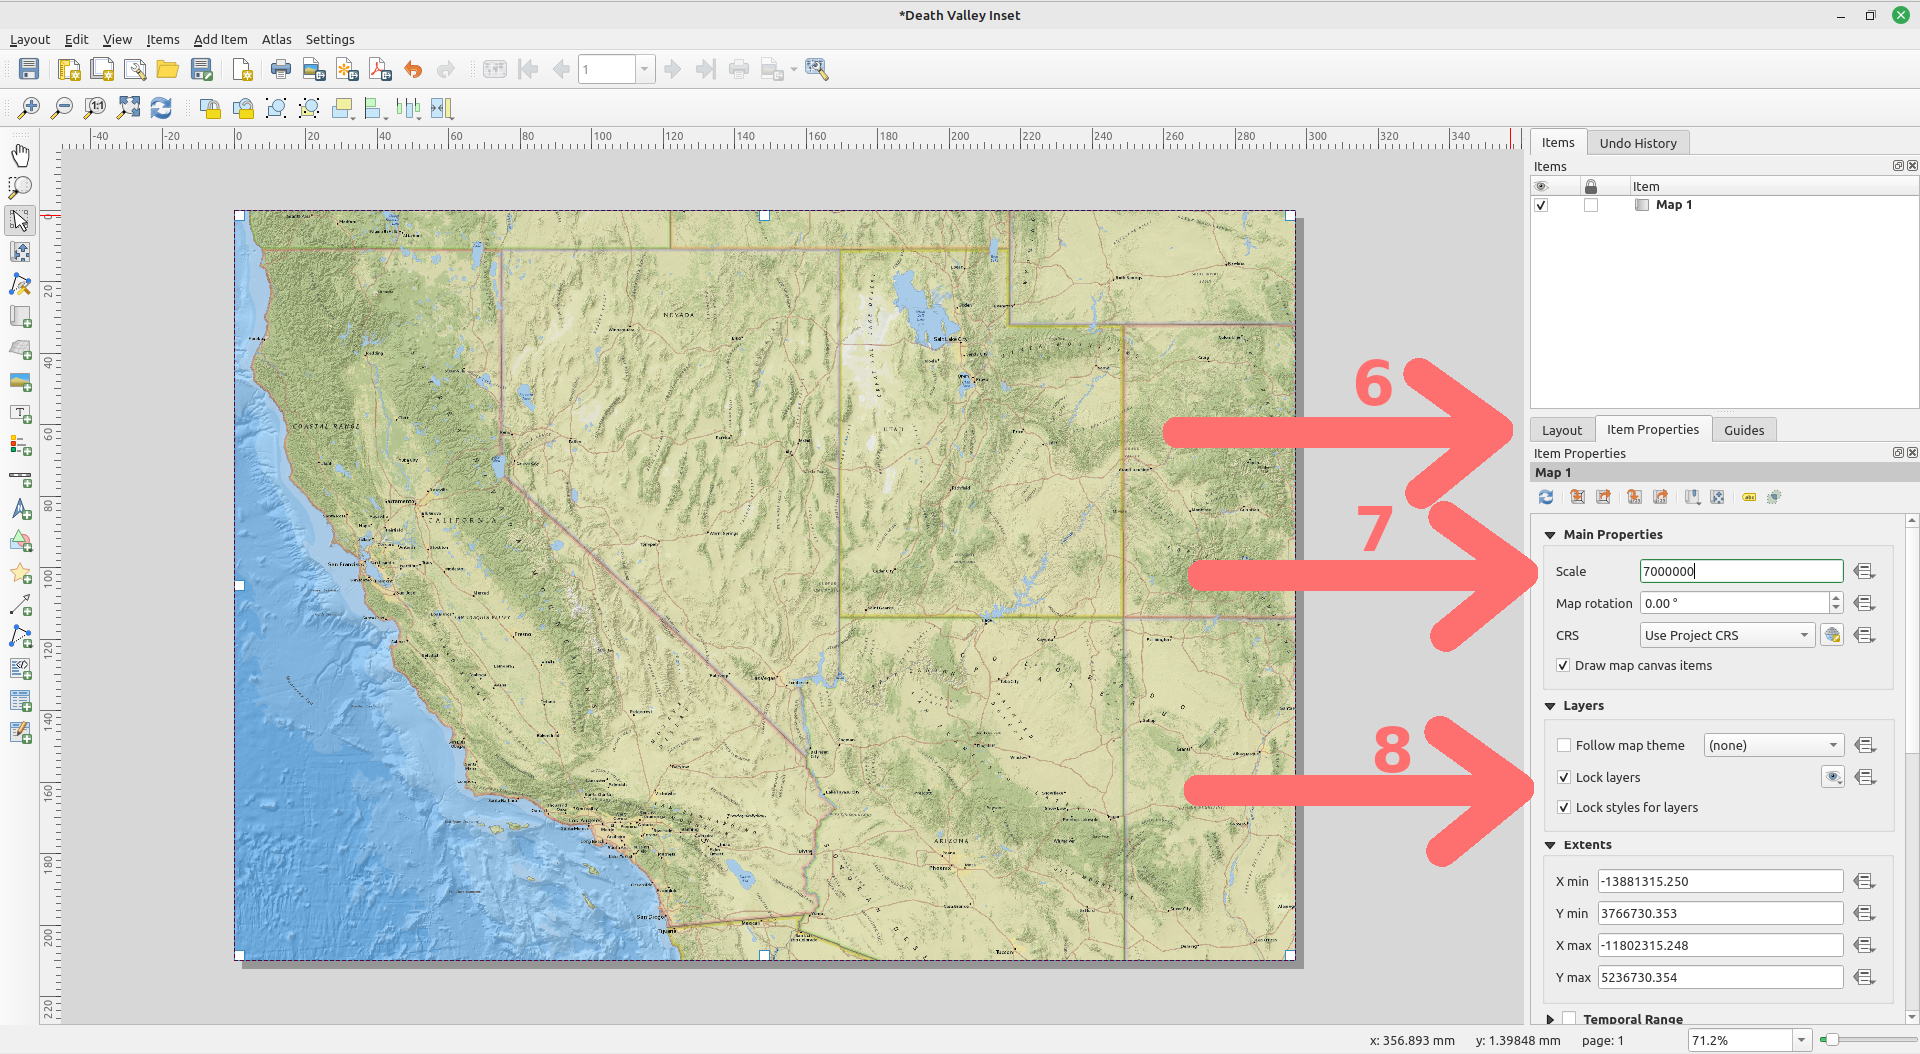
\includegraphics[width=\textwidth]{InsetItem.png}}

5. Now, select the menu \textit{Add Item}, then \textit{Add Map}. Start at one corner of the white rectangle window and drag to the opposite diagonal corner to set the map space. You will see that the rectangle window will be rendered with the map from the main QGIS canvas.

6. Click on the \textit{Item Properties} tab.

7. Adjust the \textit{Scale}, which is the zoom level, to 7000000 and hit enter.

8. Check both \textit{Lock layers} and \textit{Lock layer styles} boxes. This will ensure that if we turn off some layers or change their styles, this view will not change.


\section{Add An Inset}

9. Let's add our map from the last tutorial as an inset to this map. First, return to the main QGIS window. Add a second basemap layer following the same instructions as above, but this time use \textit{Google Satellite}.

10. Uncheck the box next to the ESRI National Geographic layer in the \emph{Layer} window, and QGIS will keep the layer in the project, but not display any of its information.

\subsection{Importing Our ECOSTRESS Death Valley Layer From The Previous Tutorial}
11. Use the \textit{browser} window to find the folder where you saved the two land surface temperature \textit{.tif} files from the last tutorial. Double click each file to add them to your map.

12. Adjust the symbology for each of the land surface temperature layer by right clicking on the layer name in the \textit{Layers} window and select \textit{Layer Properties}. On the menu bar to the left select \textit{Symbology} and change the \textit{Render type} to Singleband pseudocolor. Use the red color ramp and remember to match the minimum and maximum values from the surface temperature: 306.82 as the minimum and 347 as the maximum for both layers. Click \textit{Apply} for each layer to save the change.

\centerline{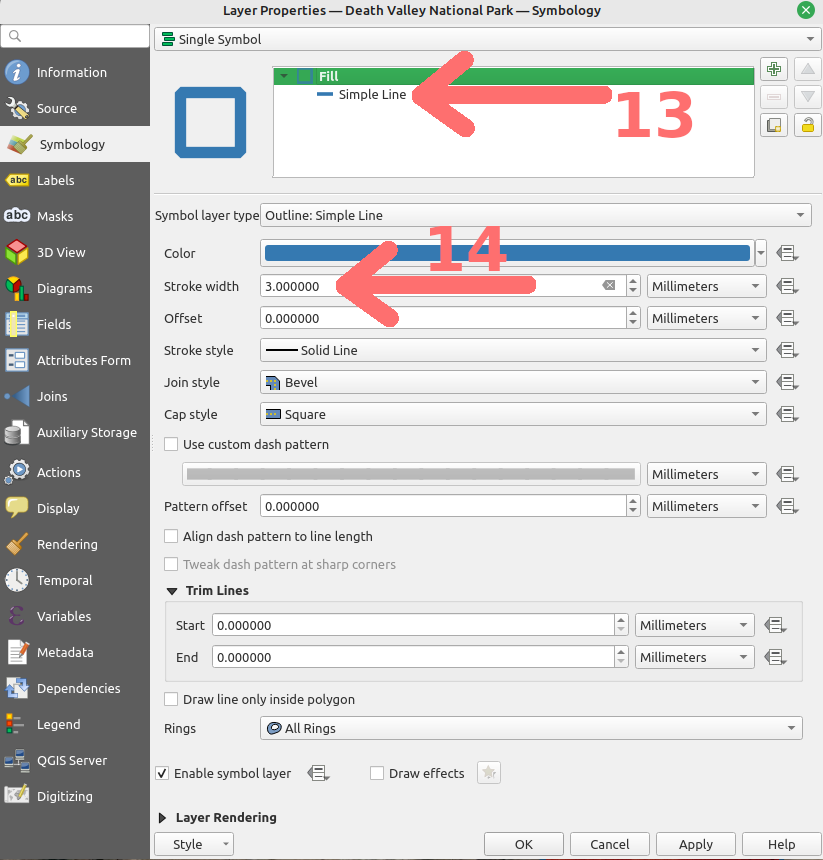
\includegraphics[width=.625\textwidth]{DVlines.png}}

13. Add in the border from the \textit{DeathValleyNationalPark.zip} shapefile. In the \textit{Browser} window, expand the zip file using the small arrow next to the filename. Double click on \textit{Death Valley National Park.shp} to add the layer. Right click on the layer in the \textit{Layers} window and change its symbology to \textit{outline blue}. 

14. The outline of the border is a little thin; let's make it thicker. First, click on the \textit{Simple Line} selection in the dialog box. Change the \textit{Stroke width} to 3 mm. Click the \textit{Apply} button at the bottom of the window.

15. Zoom in so that the outline of Death Valley National Park fits nicely in the window, it should look like this:

\vspace{.25em}

\centerline{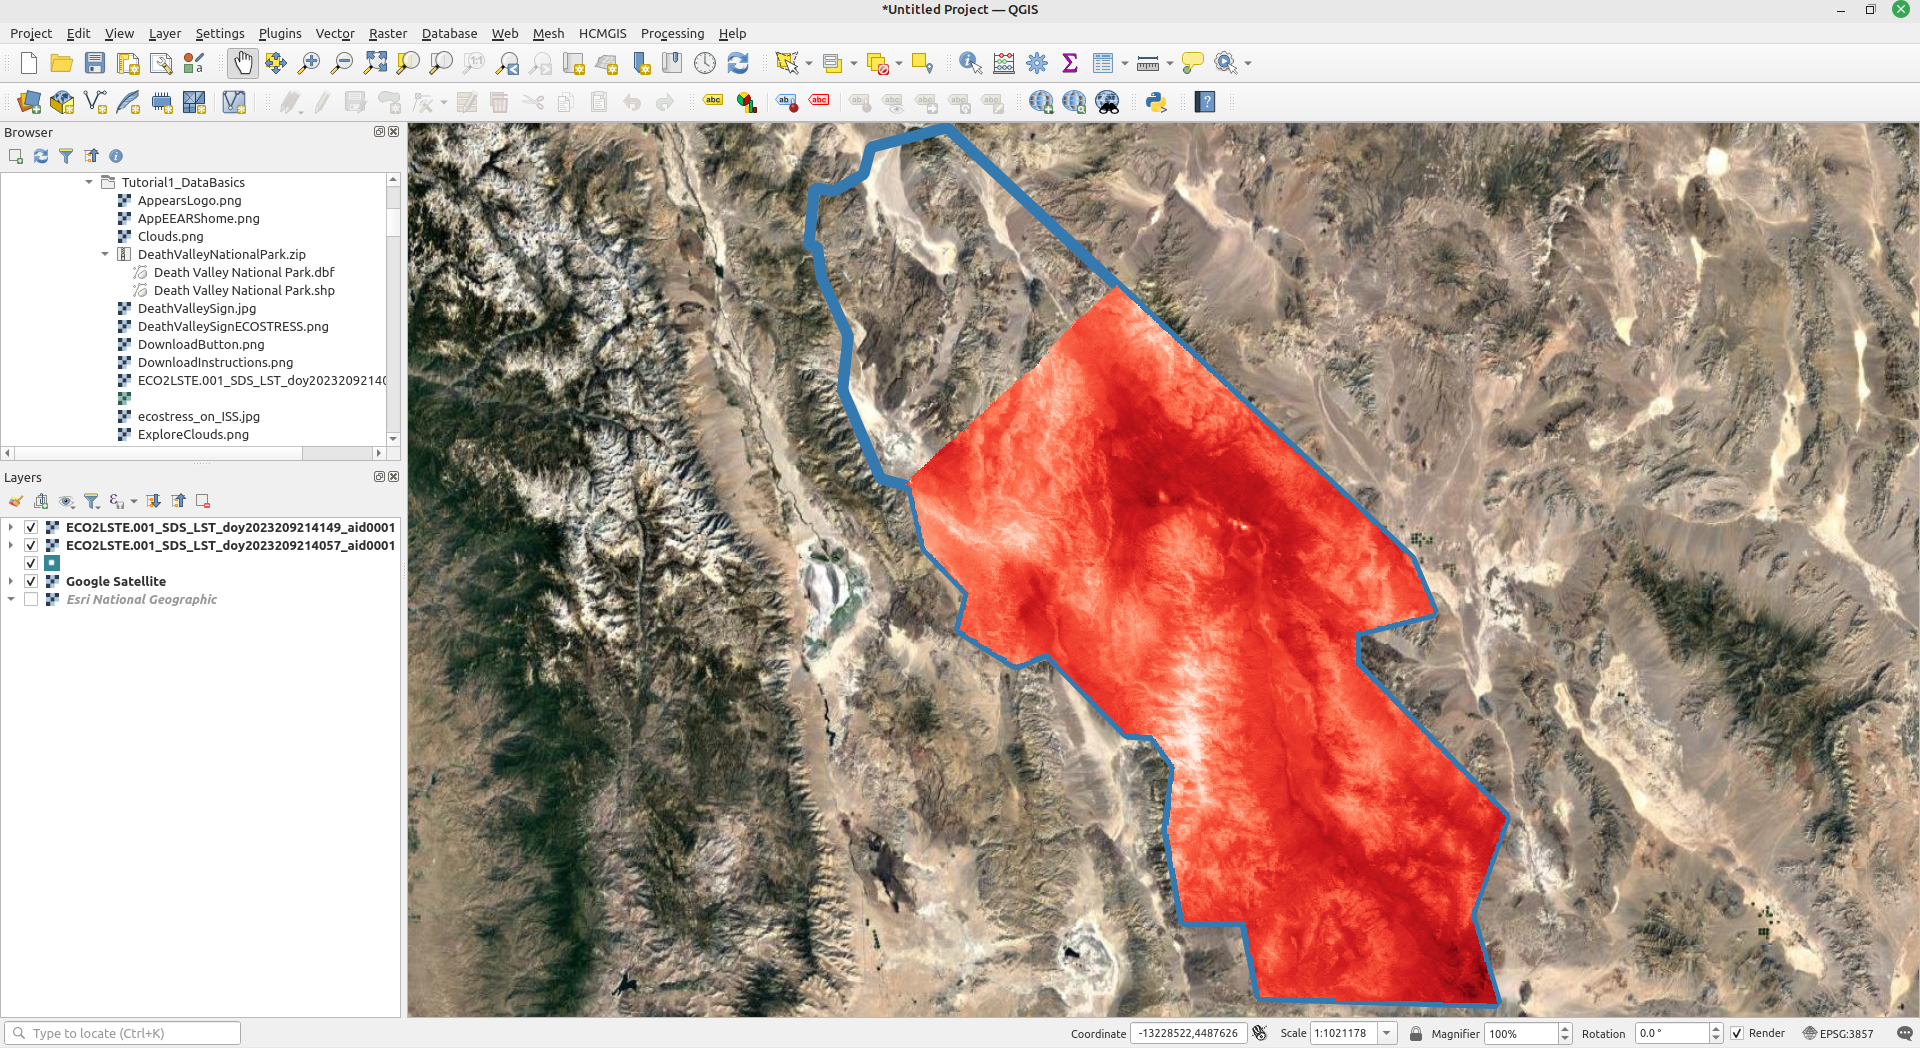
\includegraphics[width=\textwidth]{DV_LST.png}}

\subsection{Adding in our Land Surface Temperature Map as an Inset}

16. Now that we have the map how we like it the main window, switch back to the Print Layout window. Select the menu \textit{Add Item}, then \textit{Add Map}. Click and create an inset of the land surface temperature to the East of California.

\begin{tcolorbox}[enhanced jigsaw,breakable,pad at break*=1mm,
  colback=yellow!5!white,colframe=IceCreamLeaf,title=Inset Maps]
  An inset map is a smaller map within a larger map and can serve multiple purposes depending on your goals. Some things they can do:
    \begin{itemize}
         \item Provide context by showing the larger geographic region when the main map is zoomed in to a local scale:

         \vspace{.25em}
         
         \centerline{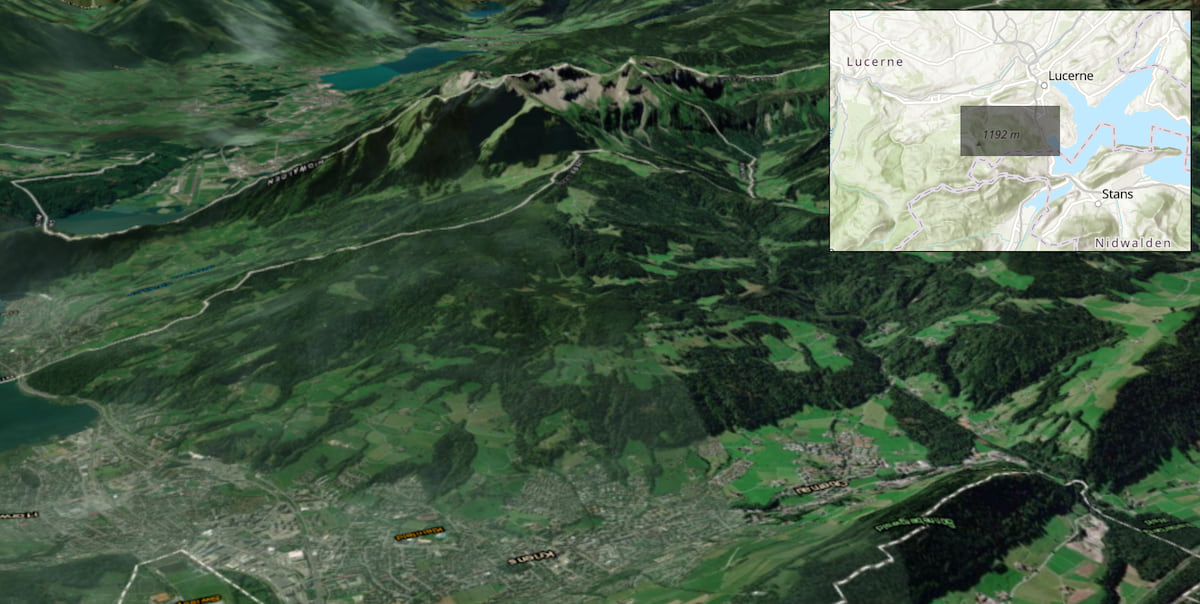
\includegraphics[width=.85\textwidth]{inset-overview.png}}

         \item Show more detail of a portion of the main map, when the main map is zoomed out to a broad scale:

         \vspace{.25em}
         
         \centerline{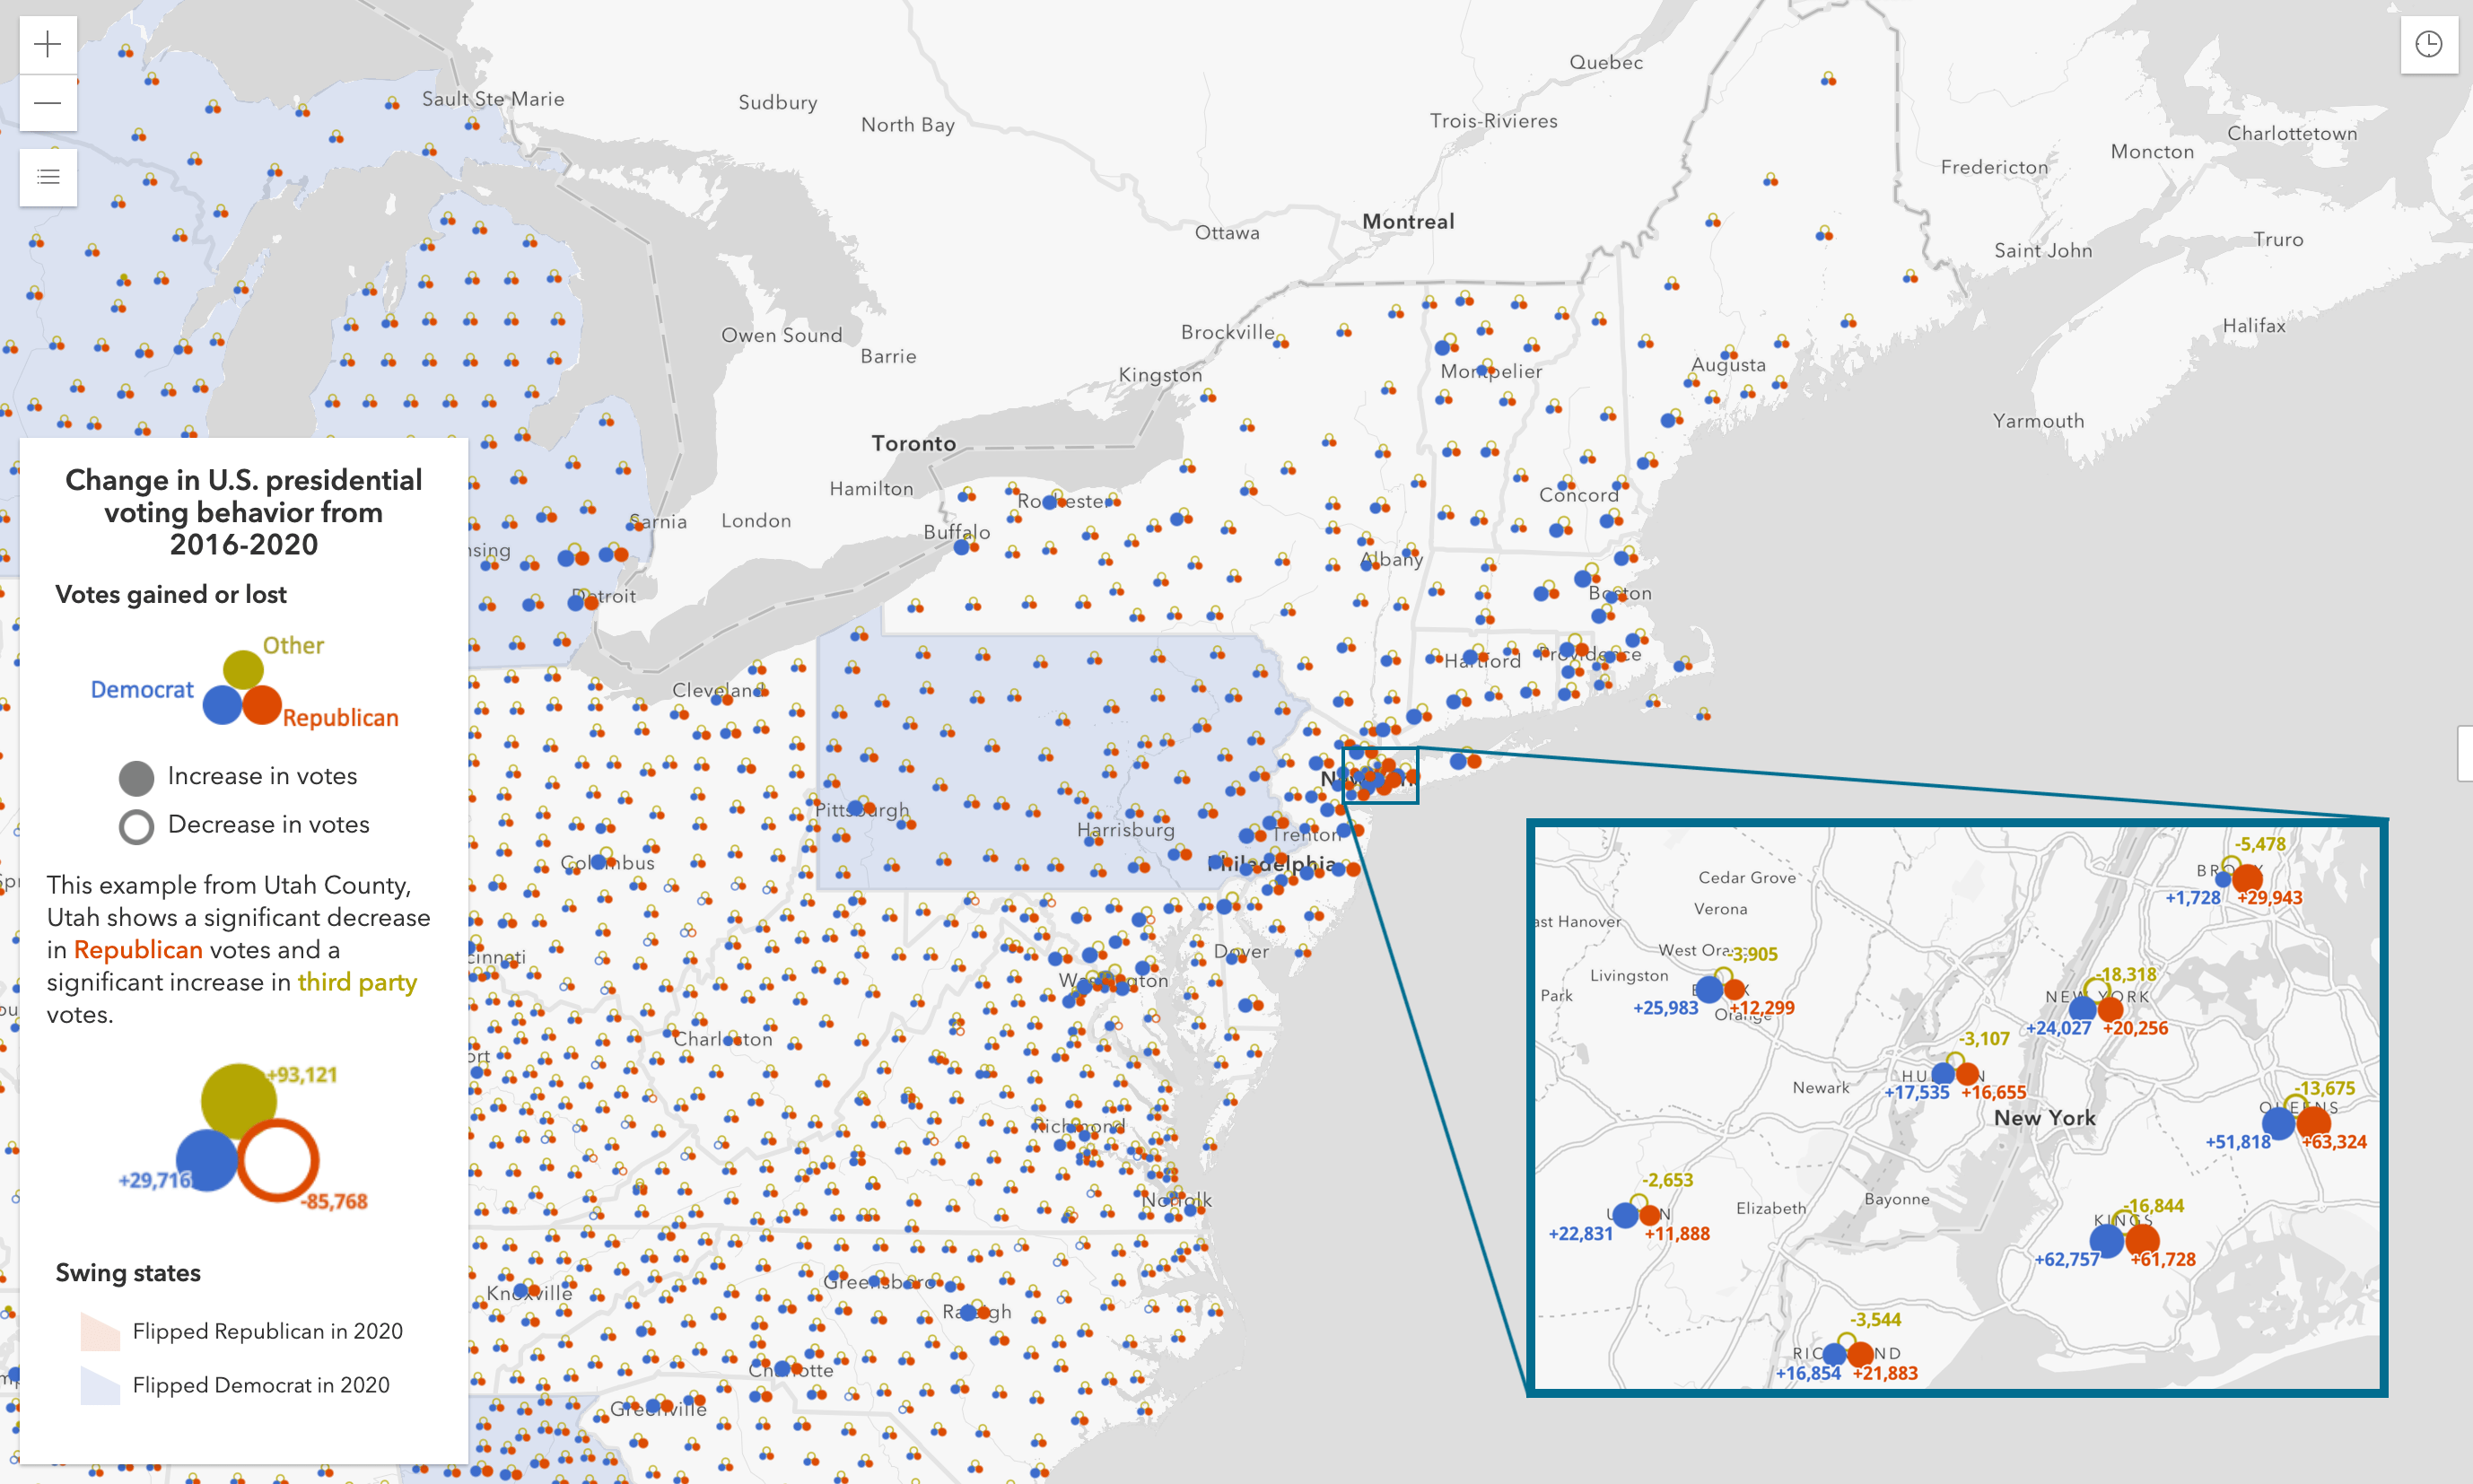
\includegraphics[width=.85\textwidth]{inset-detail.png}}

         \item Communicate additional data or information that complements the purpose of the main map:

         \vspace{.25em}

         \centerline{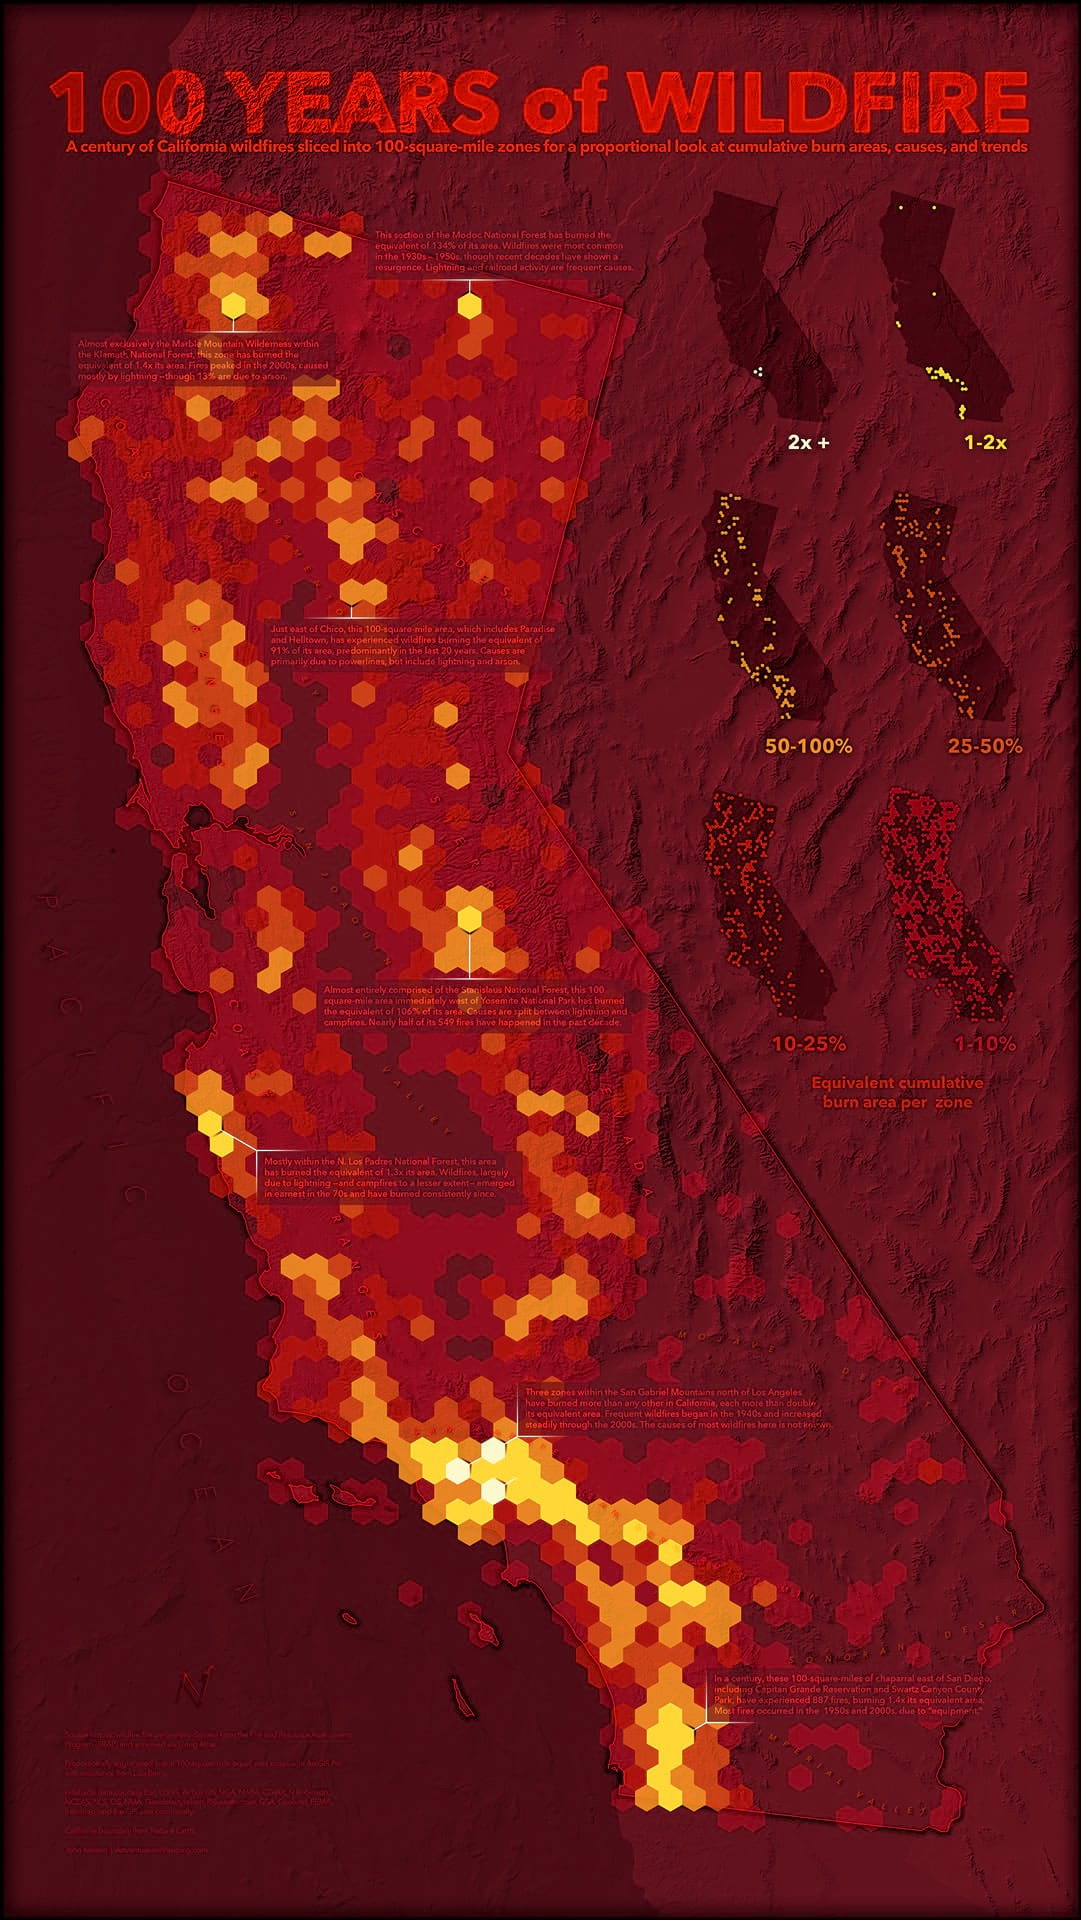
\includegraphics[width=.5\textwidth]{inset-multiples.jpg}}

         \item Display noncontiguous geographies at a single glance:

         \vspace{.25em}

         \centerline{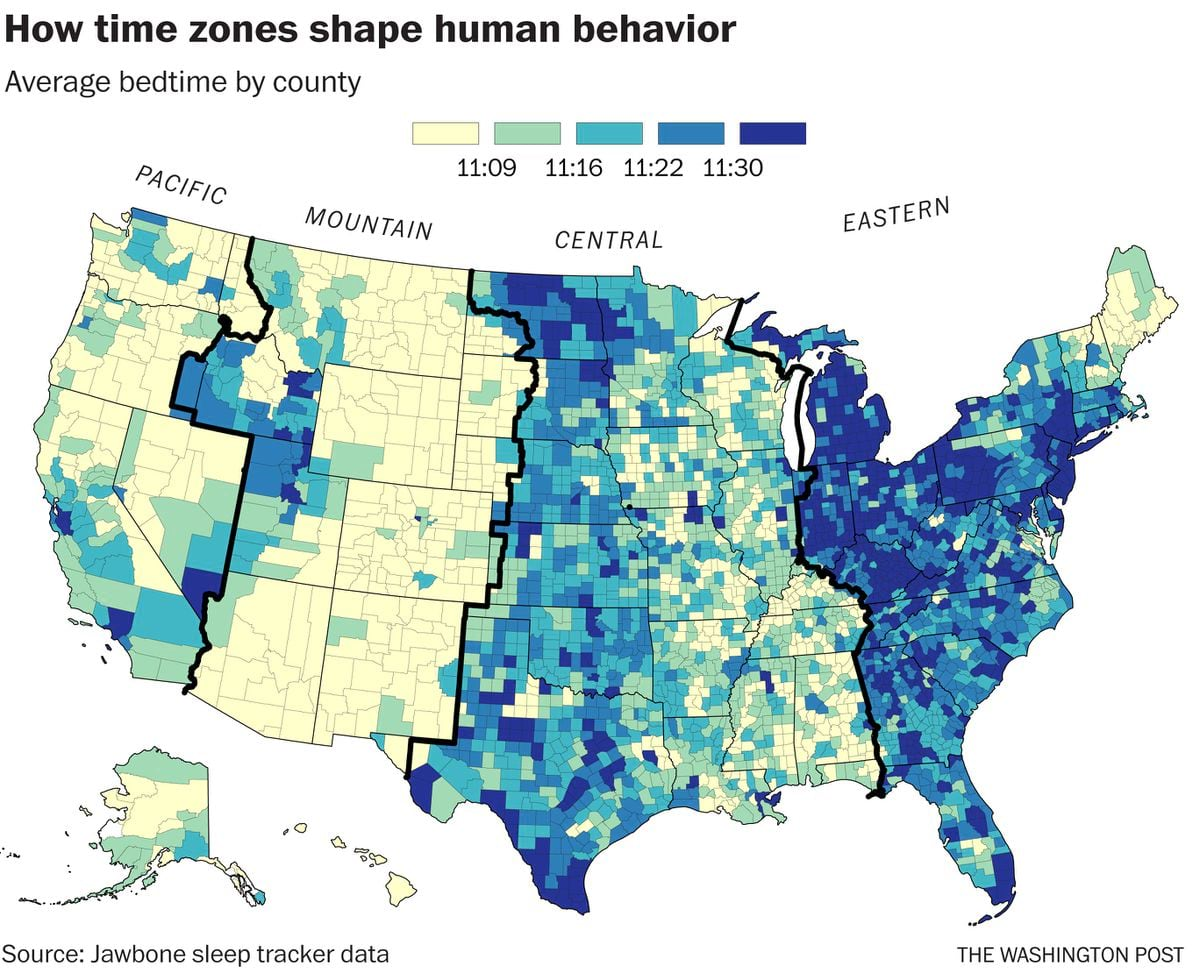
\includegraphics[width=.65\textwidth]{inset-noncontiguous.jpg}}
    \end{itemize}
\end{tcolorbox}

\vspace{.25em}

\centerline{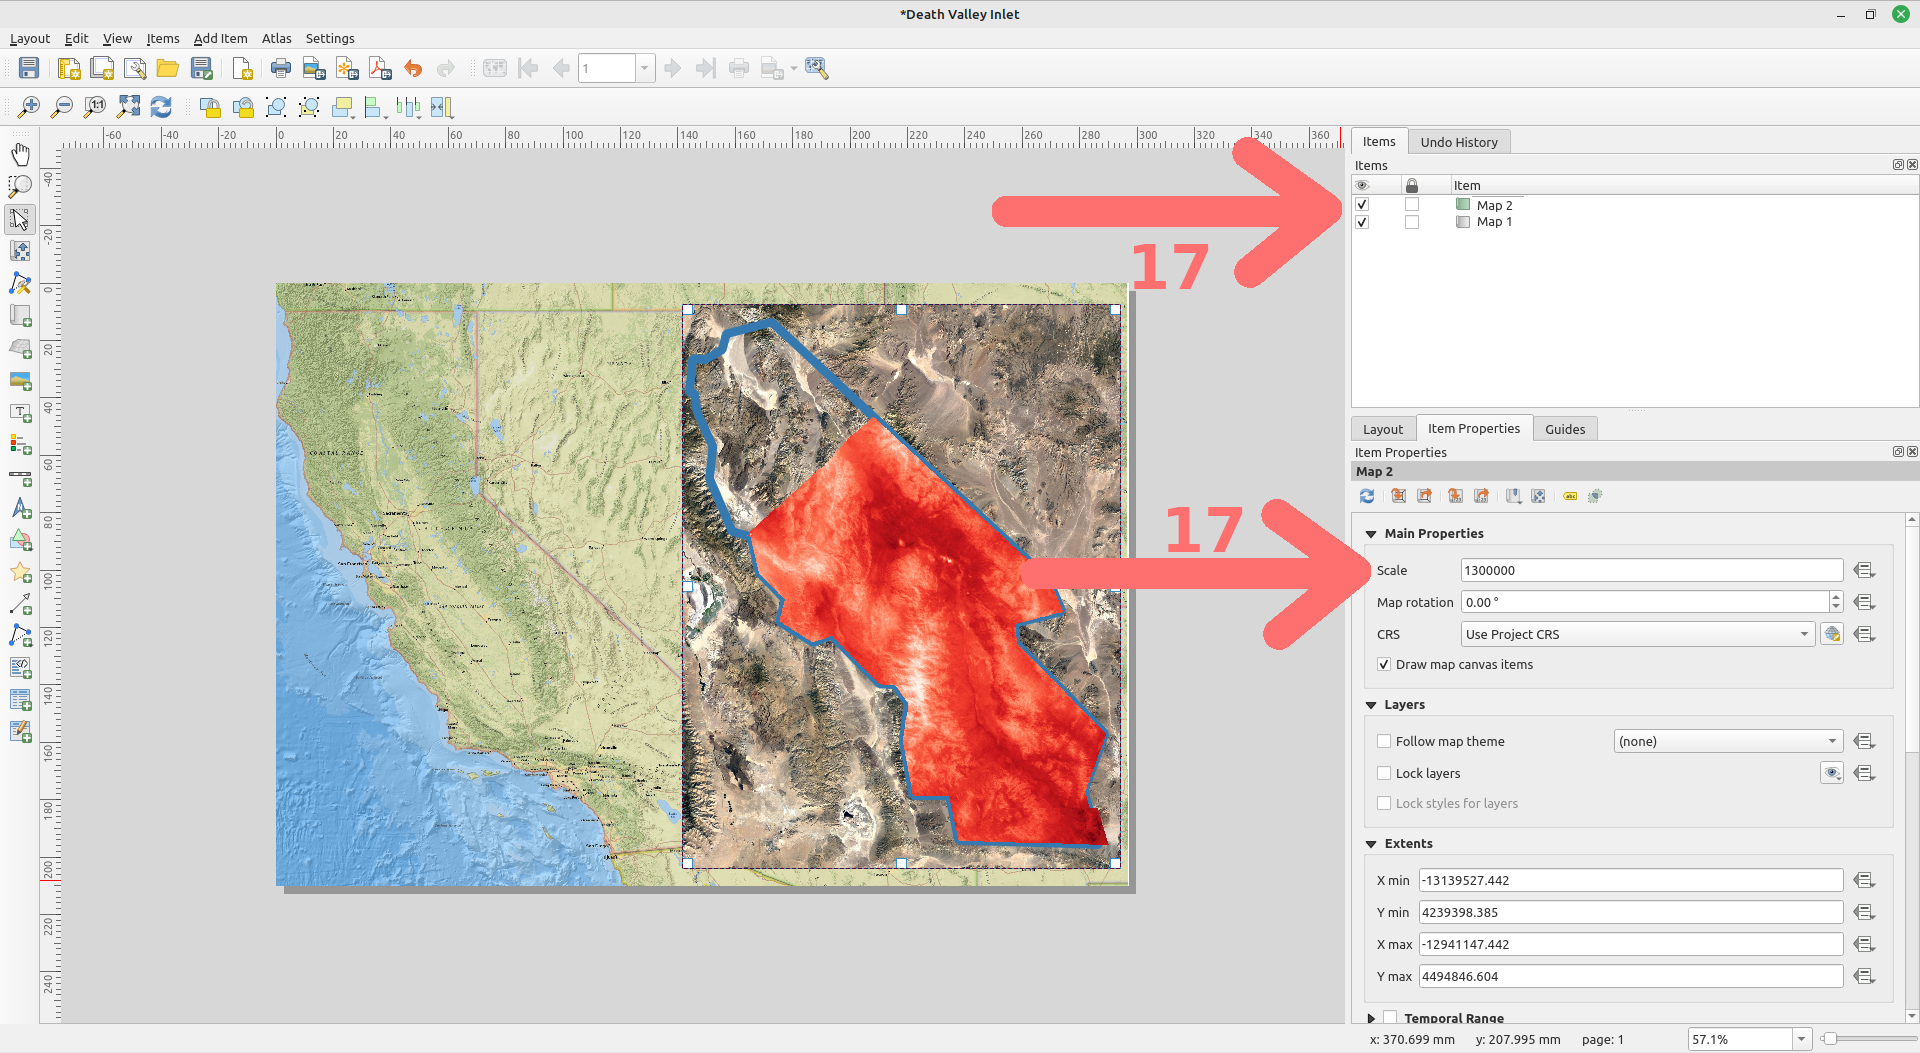
\includegraphics[width=\textwidth]{AddInset.png}}

17. Under the \textit{Item Properties} for the inset map (typically numbered \textit{Map 2} in the \textit{Items} window), change the scale to 1300000 to frame Death Valley. The scale is now fixed at 1:1300000 distance.

\vspace{.25em}

\centerline{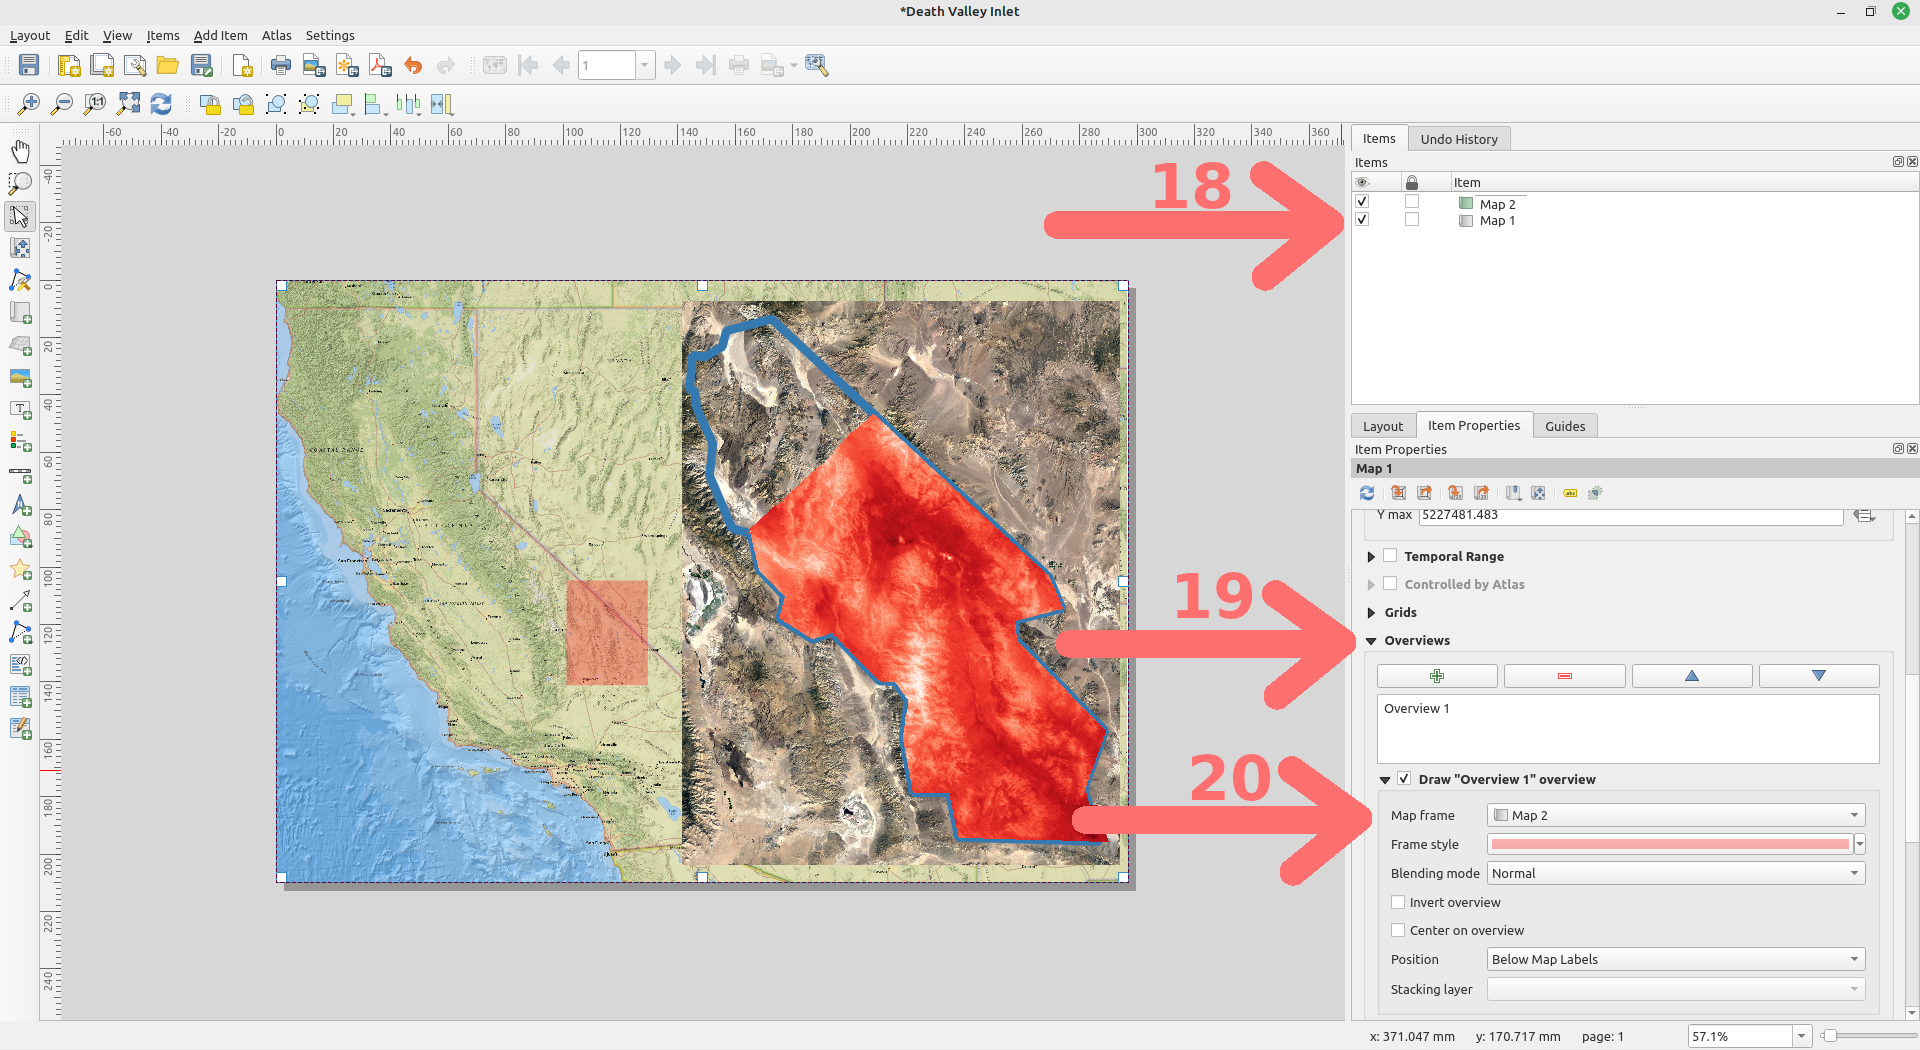
\includegraphics[width=\textwidth]{RegionShade.png}}

18. QGIS has an excellent tool for automatically highlighting the area on the main map that is represented in an inset. First, select \textit{Map 1} (or your main map number) in the \textit{Items} window.
 
19. Next, under \textit{Item Properties}, scroll down to find the \textit{Overviews} menu. Click the green plus sign to get an overview.

20. Under map frame, select \textit{Map 2} (or whatever you have named your inset map). The area from the inset should now be highlighted on the main map. Adjust the highlight color to match your mood.

\section{Using ColorBrewer In QGIS}

Choosing effective colors for maps is surprisingly tough. ColorBrewer is a tool designed to take some of the guesswork out of it by creating color schemes for your specific mapping needs. The suggested colors are based on the type of data (sequential, divergent, or qualitative). It also provides options for various display environments, such as laptop, photocopy, projector, and color-blind safe options. 

Although you can manually edit color ramps in QGIS, many of the ColorBrewer palettes are already available in QGIS through the \textit{Style Manager}. 

\vspace{1em}

21. To access the style manager, open QGIS and select \textit{Settings}, then \textit{Style Manager}.

22. Select \textit{Color Ramps}

23. Use the ``+'' sign to select \textit{Catalog: ColorBrewer}.

\centerline{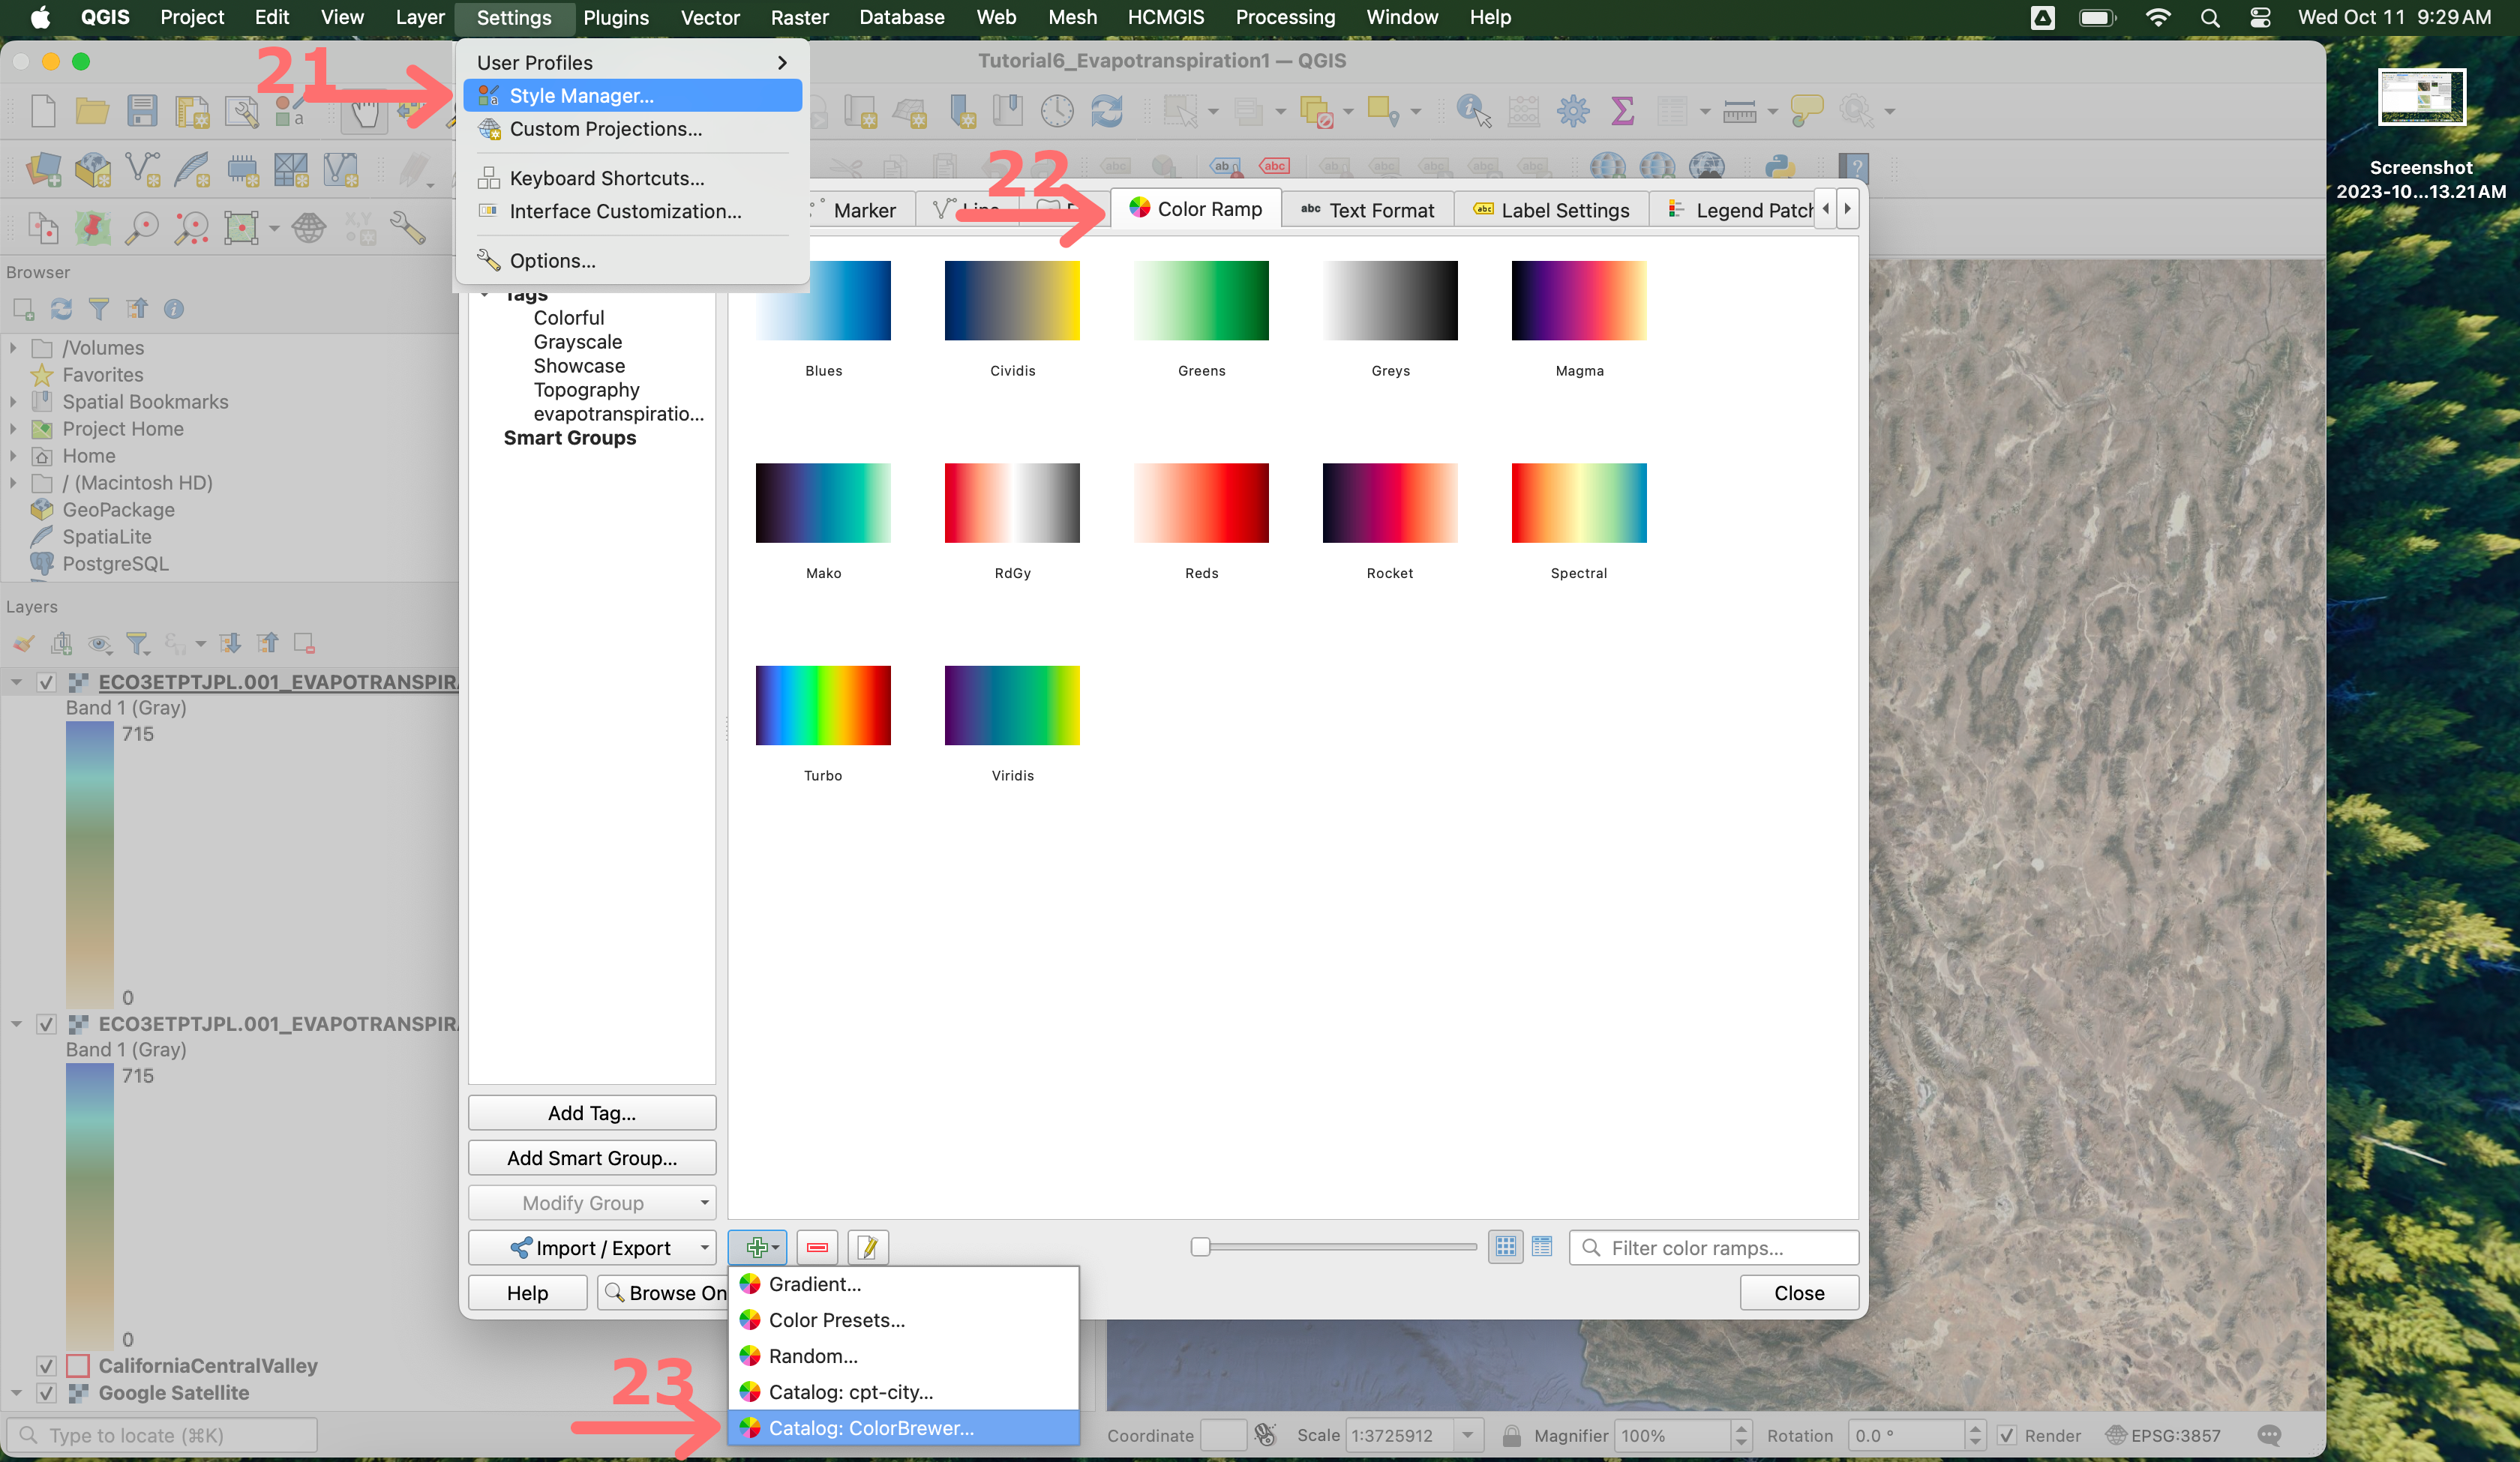
\includegraphics[width=.87\textwidth]{StyleManager.png}}

\vspace{.5em}

\centerline{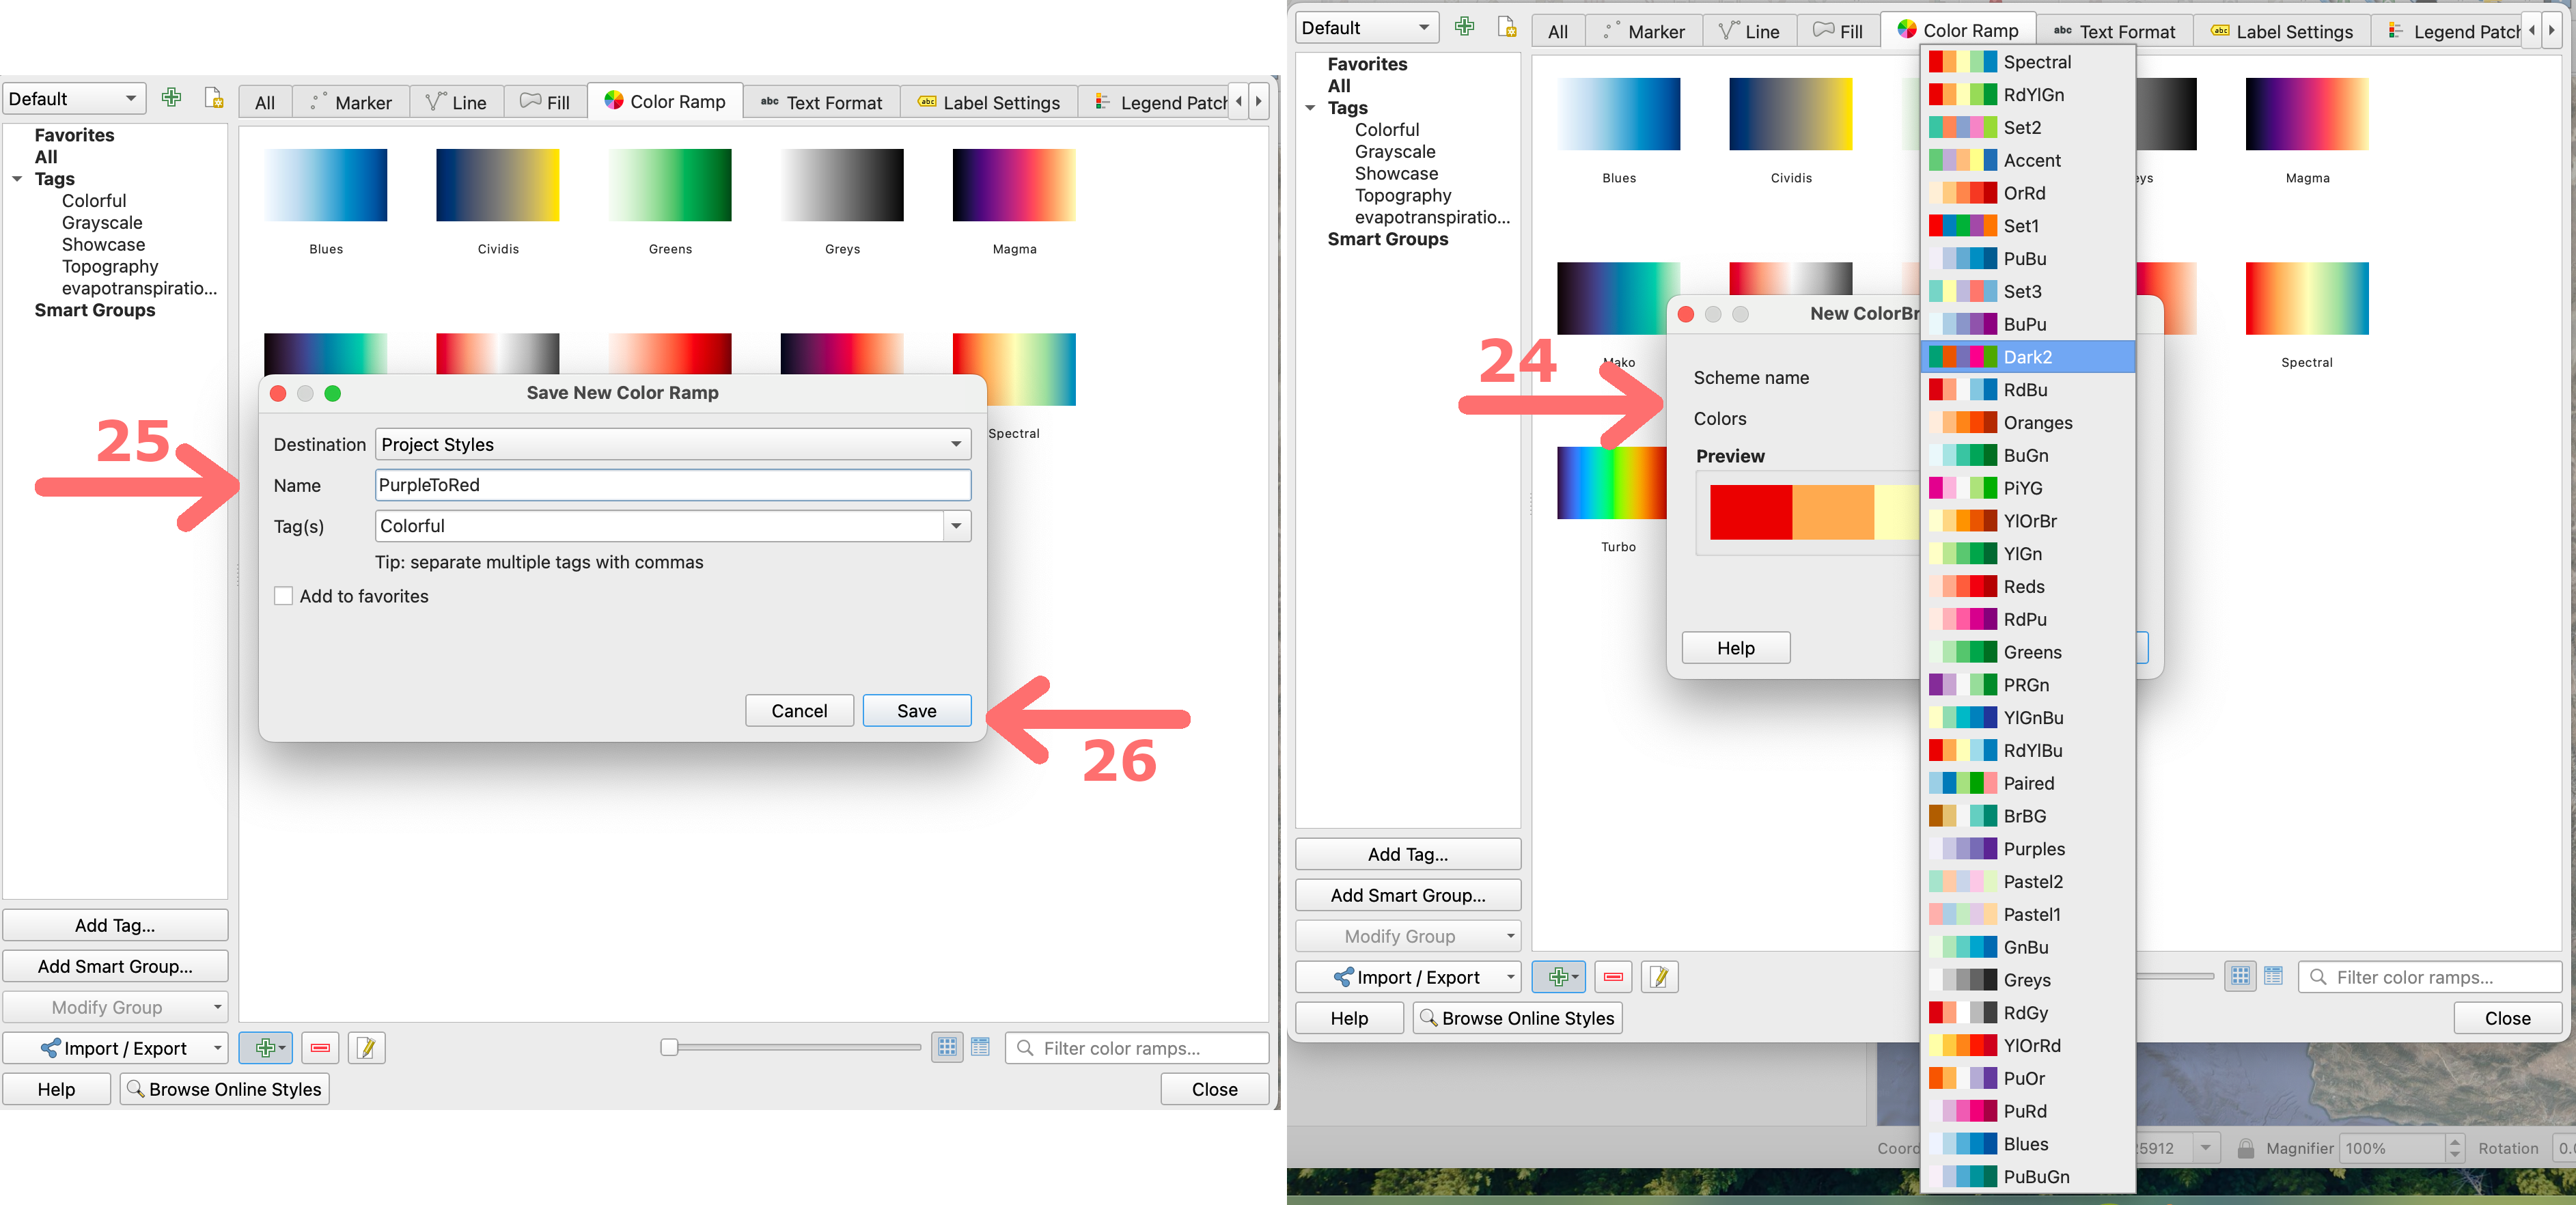
\includegraphics[width=.87\textwidth]{QGIScolorBrewer.png}}

\vspace{.5em}

24. From this screen, you can select from preset color schemes and the number of color classes you want.

25. After you click \textit{OK}, QGIS prompts you to name and save your new color ramp. Pick a name that you can remember. If you think you will use this color ramp often, you can click on the ``Add to favorites'' box. 

26. Click \textit{Save}.

27. This color ramp can now be accessed by right clicking on a layer, selecting the \textit{Symbology} tab, then the little down arrow next to the color ramp bar. Under the heading ``All Color Ramps'' you should find your new ramp. See the screen shot below for where to look. NOTE: If you have marked it as a favorite, it shows up in the first list. 

\centerline{\includegraphics[width=.87\textwidth]{UseColorRamp.png}}

\vspace{.5em}

\begin{tcolorbox}[colback=yellow!5!white,colframe=MACred,title= \vspace{.2em} \Large Make a Map Assignments]
	\addcontentsline{toc}{section}{Map of the Week Assignments}
	\large
	\begin{enumerate}
		\item Read the article \href{https://jeremydforsythe.github.io/icecream-tutorials/Tutorial12_MakingBetterMaps/ColorBrewer.pdf}{ColorBrewer.org: An Online Tool for Selecting Colour
Schemes for Maps}.
            \item Redesign a previous map, using the principles of graphical communication:
	    \begin{itemize}
		      \item What are the variables your map displays, and what visual dimensions are you using to encode that data? What color palette are you using and why?
		      \item What is your data/ink ratio? Do you have unnecessary lines? Can your line strokes be reduced in weight? What are you using as your base map and why?
		      \item What \href{https://en.wikipedia.org/wiki/Map_layout}{map layout }are you using? Are the panels the same size? Similarly justified? Do they have titles and captions that explain their contents? Is there a hierarchy of size in the type?
            \end{itemize}
    \item Once you have redesigned your map, trade with one of your classmates and discuss the choices you made in your redesign. Is there anything you wish to further edit? 
    \item Find an environmental event (e.g., climate disaster) that occurred in the past week. Download relevant ECOSTRESS data (LST, ET, WUE, ESI) for that location. Make a map using best practices for data visualization. Write a 4-6 sentence paragraph (topic sentence, supporting description, relevant conclusion) describing the event to accompany the map.
	\end{enumerate}
\end{tcolorbox}

\begin{tcolorbox}[colback=yellow!5!white,title=\textbf{Datafiles}]
	\addcontentsline{toc}{section}{Datafiles}
	\large
	In case you encountered any issues with the A$\rho\rho$EEARS database, here are copies of the ECOSTRESS GeoTIFF files for Death Valley:
	\begin{enumerate}
		\item \href{https://jeremydforsythe.github.io/icecream-tutorials/Tutorial3_AccessingRemoteSensingDataWithAppears/ECO2LSTE.001_SDS_LST_doy2023209214149_aid0001.tif}{\small ECO2LSTE.001\textunderscore SDS\textunderscore LST\textunderscore doy2023209214149\textunderscore aid0001.tif}
		\item \href{https://jeremydforsythe.github.io/icecream-tutorials/Tutorial3_AccessingRemoteSensingDataWithAppears/ECO2LSTE.001_SDS_LST_doy2023209214057_aid0001.tif}{\small ECO2LSTE.001\textunderscore SDS\textunderscore LST\textunderscore doy2023209214057\textunderscore aid0001.tif}
	\end{enumerate}
\end{tcolorbox}

%%%%%%%%%%%%%%%%%%%%%%%%%%%%%%%%%%%%%%%%%%%%%%%%%%%%%%%%%%%%%%%%%%%%%%%%%%%%%%%%%%% End of Document
\vfill

\hrule

\vspace{1em}

\small \textbf{Recommended Citation:} Forsythe, J.D., G.R. Goldsmith, and J.B. Fisher. 2023. Observing Earth from Above Tutorials. Chapman University. \url{https://jeremydforsythe.github.io/icecream-tutorials/}

\vspace{1em}

This work is supported by funding from NASA ECOSTRESS Mission Grant \#80NSSC23K0309 (I.C.E. C.R.E.A.M.: Integrating Communication of ECOSTRESS Into Community Research, Education, Applications, and Media) and is openly licensed via \href{https://creativecommons.org/licenses/by-nc/4.0/}{CC BY-NC}.

\end{document}
